\paragraph{Trajectory} \label{sec:TrajectoryDesign}

\begin{sidewaysfigure}[h!]
	\centering
	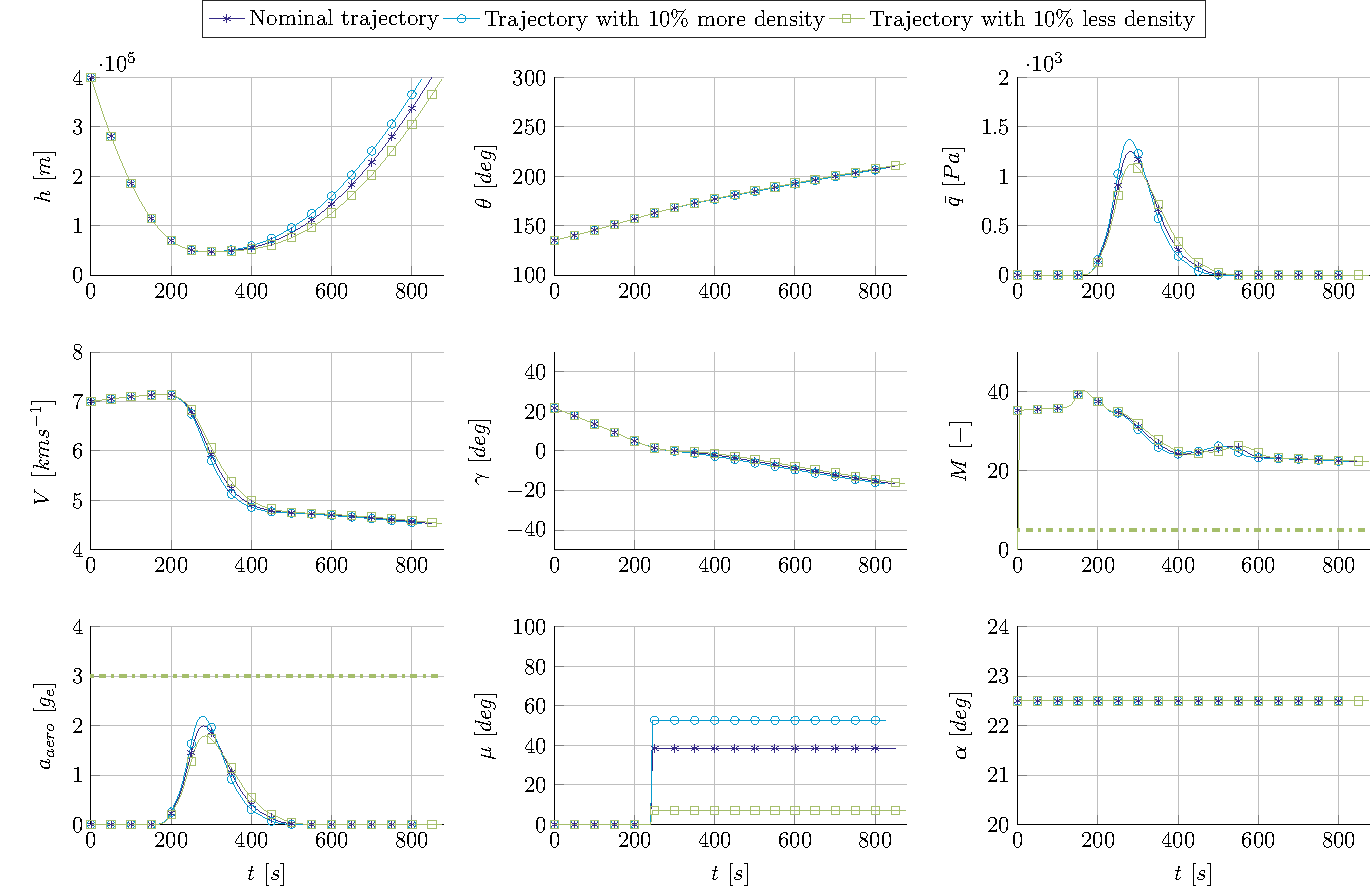
\includegraphics[width=0.95\textwidth]{Figure/Orbit/sensitivity_aerocapture.pdf}
	\caption{ Results of the re-entry trajectory for three different density profiles. The trajectories with modified density are corrected to maintain the same exit velocity. The horizontal dashed lines are design limits (for the \gls{sym:M} and \gls{sym:acc} plots) }
	\label{fig:orbit_aerocapture_data}
\end{sidewaysfigure}


\paragraph{Aerodynamic shape} \label{sec:AeroDesign}
 The aeroshell will have a shape similair to configuration D described in section \ref{sec:aeroshapes}, with a radius of 6 meters and a half cone angle of approximately $\gls{sym:theta} = XX\deg$. The curved nose will have an outer radius of $2.5m$. The cross section offset at the rear of the body is approximately $0.91m$. At an angle of attack of $\gls{sym:alpha} = 22.5\deg$, it has a lift to drag ratio of $\gls{sym:L}/\gls{sym:D} = 0.35$ and a drag coefficient of $\gls{sym:CD} = 1.3$. At this angle of attack, a \gls{cg} offset of $\gls{sym:CML}/\gls{sym:CX} = 0.5m$ is required to trim the vehicle around its pitch axis. It has a moment derivative of $\gls{sym:cm-alpha} = -0.21$. 
 
 Figures \ref{fig:aeroshape.iso} through \ref{fig:aeroshape.top} 
 

\paragraph{Structural analysis and design}


The inflatable consists of ten toroids, stacked aside and on top of one another. The asymmetric shape obtained by aerodynamic optimization is attained by arranging the toroids at an angle with respect to one another. The result is an assembly of circular inflatables, placed at differing radial distances with respect to the centerbody. While the structural performance of the inflatable is altered, an asymmetric configuration is achieved by stitching the toroids and varying the radial length of the straps over the sphere cone circumference. Structural performance is altered in the sense that the asymmetry of the configuration implies additional concerns for aeroelasticity phenomena, such as limit cycle oscillations, for example. These phenomena, however, are highly unpredictable and warrant additional wind tunnel and flight testing in any case. 

The number of toroids is based on Figure \ref{fig:inflpress_strucmass}, which shows that mass decreases beyond ten toroids are insignificant. Moreover, ten toroids are sufficient to adequately represent the optimized aerodynamic shape. 

Structural loads are carried by fibres, interlaced warp and weft to provide load-carrying capability in all required directions: circumferential and hoop. As such,fibres are woven perpendicular to each other. To this end, a plain weave pattern is adequate. The low mechanical properties typically attributed to such a plain weave are not an issue, based on the following reasoning.

Key driver for the design case at hand is the minimum material thickness: the loading was thusly low that the required thickness to withstand loads induced by aerodynamic and inflation pressure is lower than minimum gage thicknesses. To this end, fiber weight performance is mainly dictated by density and minimum gage thickness. The flexible material mass achieved by Spectra 2000, expected to perform best of all fibres given its low density of 970 [$kg \cdot m^{-3}$], compared to Kevlar's 1440 [$kg \cdot m^{-3}$], is 20 [$kg$] lower than that achieved by Kevlar 49 and the other fibers, of comparable density. 

Preference is given to Kevlar 49, however, for two reasons. Firstly, it is widely commercially available and has been applied for a longer number of years, with resulting lower costs associated with its fabrication and application. Secondly, it has been previously applied for inflatable re-entry vehicles, namely in the \gls{irve} missions \cite{Hughes2011}. Spectra 2000 therefore introduces additional costs and technical risks that offset the weight advantage offered. Moreover, the weight advantage does not further the entry vehicle in the sense that supplementing another crew member is out of reach and requirements are respected. Other fibers are comparable to Kevlar in their performance, with none of the benefits of past application in \glspl{hiad}.

Based on the parametric mass model and the inherent stress equations, the minimum gage thickness of 0.125 [$mm$] is deemed attainable. Such a minimum thickness is achievable for a plain weave, based on its proposed application in \gls{irve}-4 in a 0.127 [$mm$] lay-up \cite{Litton2011} and commercial availability of these weave patterns\footnote{URL:\url{http://www.cstsales.com/aramid_fabric.html}. Accessed: 16-06-2015}. 

The structural feasibility thereof is ascertained by the truss-based analysis model. The truss-based analysis model uses the representation in Figure \ref{fig:strucreps}. Cross-sections that displayed the most extreme loading are the short side, defined at the inflatable minimum diameter, and the long side, defined at the inflatable maximum diameter. Due to the skewness, load asymmetry is introduced which is thereby evaluated by some extent through evaluation of multiple cross-sections.

\begin{figure}[h!]
	\centering

	\begin{subfigure}[b]{0.45\textwidth}
		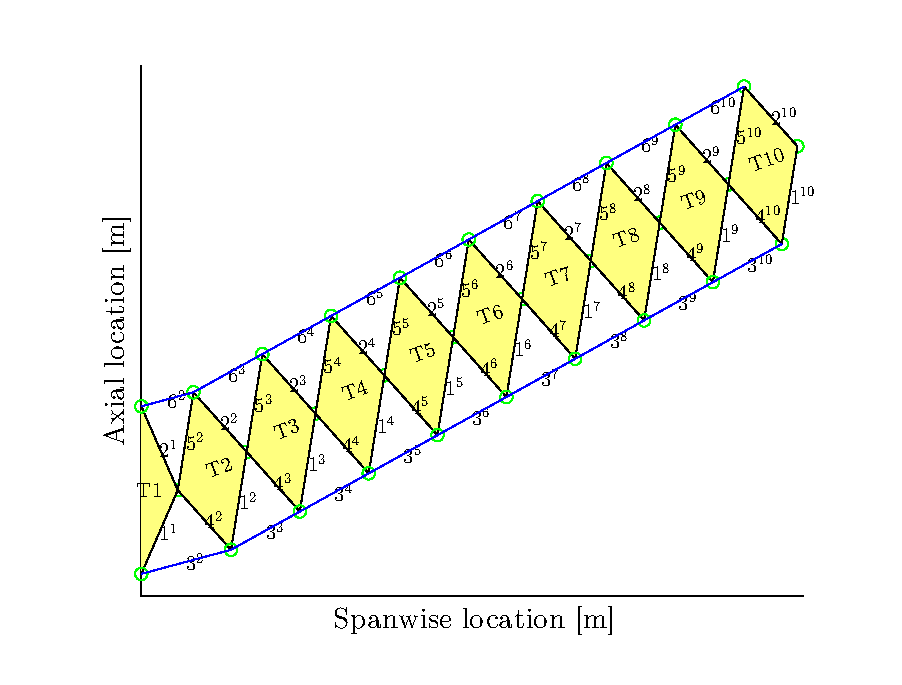
\includegraphics[width=0.96\textwidth]{./Figure/Structure/shape_long.eps}
		\caption{Cross-sectional view at maximum diameter}
		\label{fig:shapel}
	\end{subfigure}
	\begin{subfigure}[b]{0.45\textwidth}
		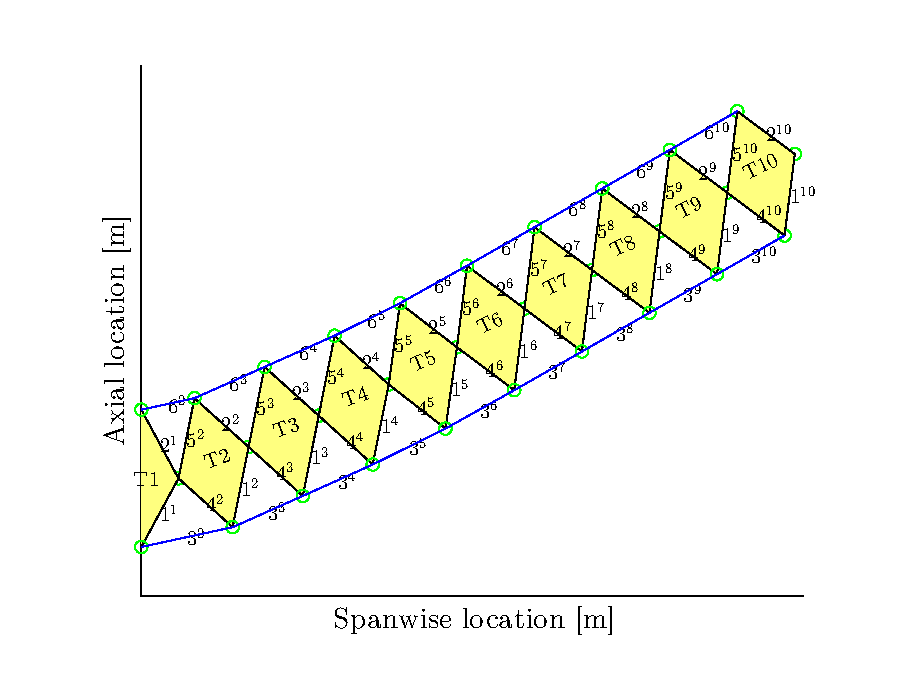
\includegraphics[width=0.96\textwidth]{./Figure/Structure/shape_short.eps}
		\caption{Cross-sectional view at minimum diameter}
		\label{fig:shapes}
	\end{subfigure}
\begin{subfigure}[c]{0.5\textwidth}
		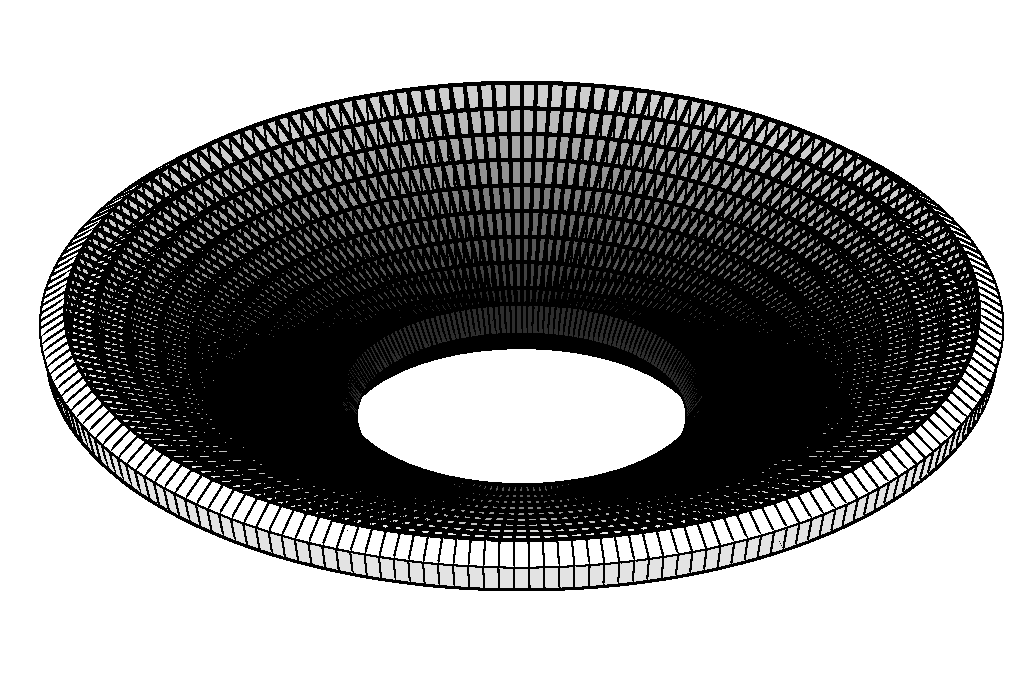
\includegraphics[width=0.96\textwidth]{./Figure/Structure/struc_rep.eps}
		\caption{Isometric view}
		\label{fig:iso}
	\end{subfigure}
\caption{Structural representation of inflatable structure}
\label{fig:strucreps}
\end{figure}

\begin{figure}[h!]
		\hspace{-16mm}
		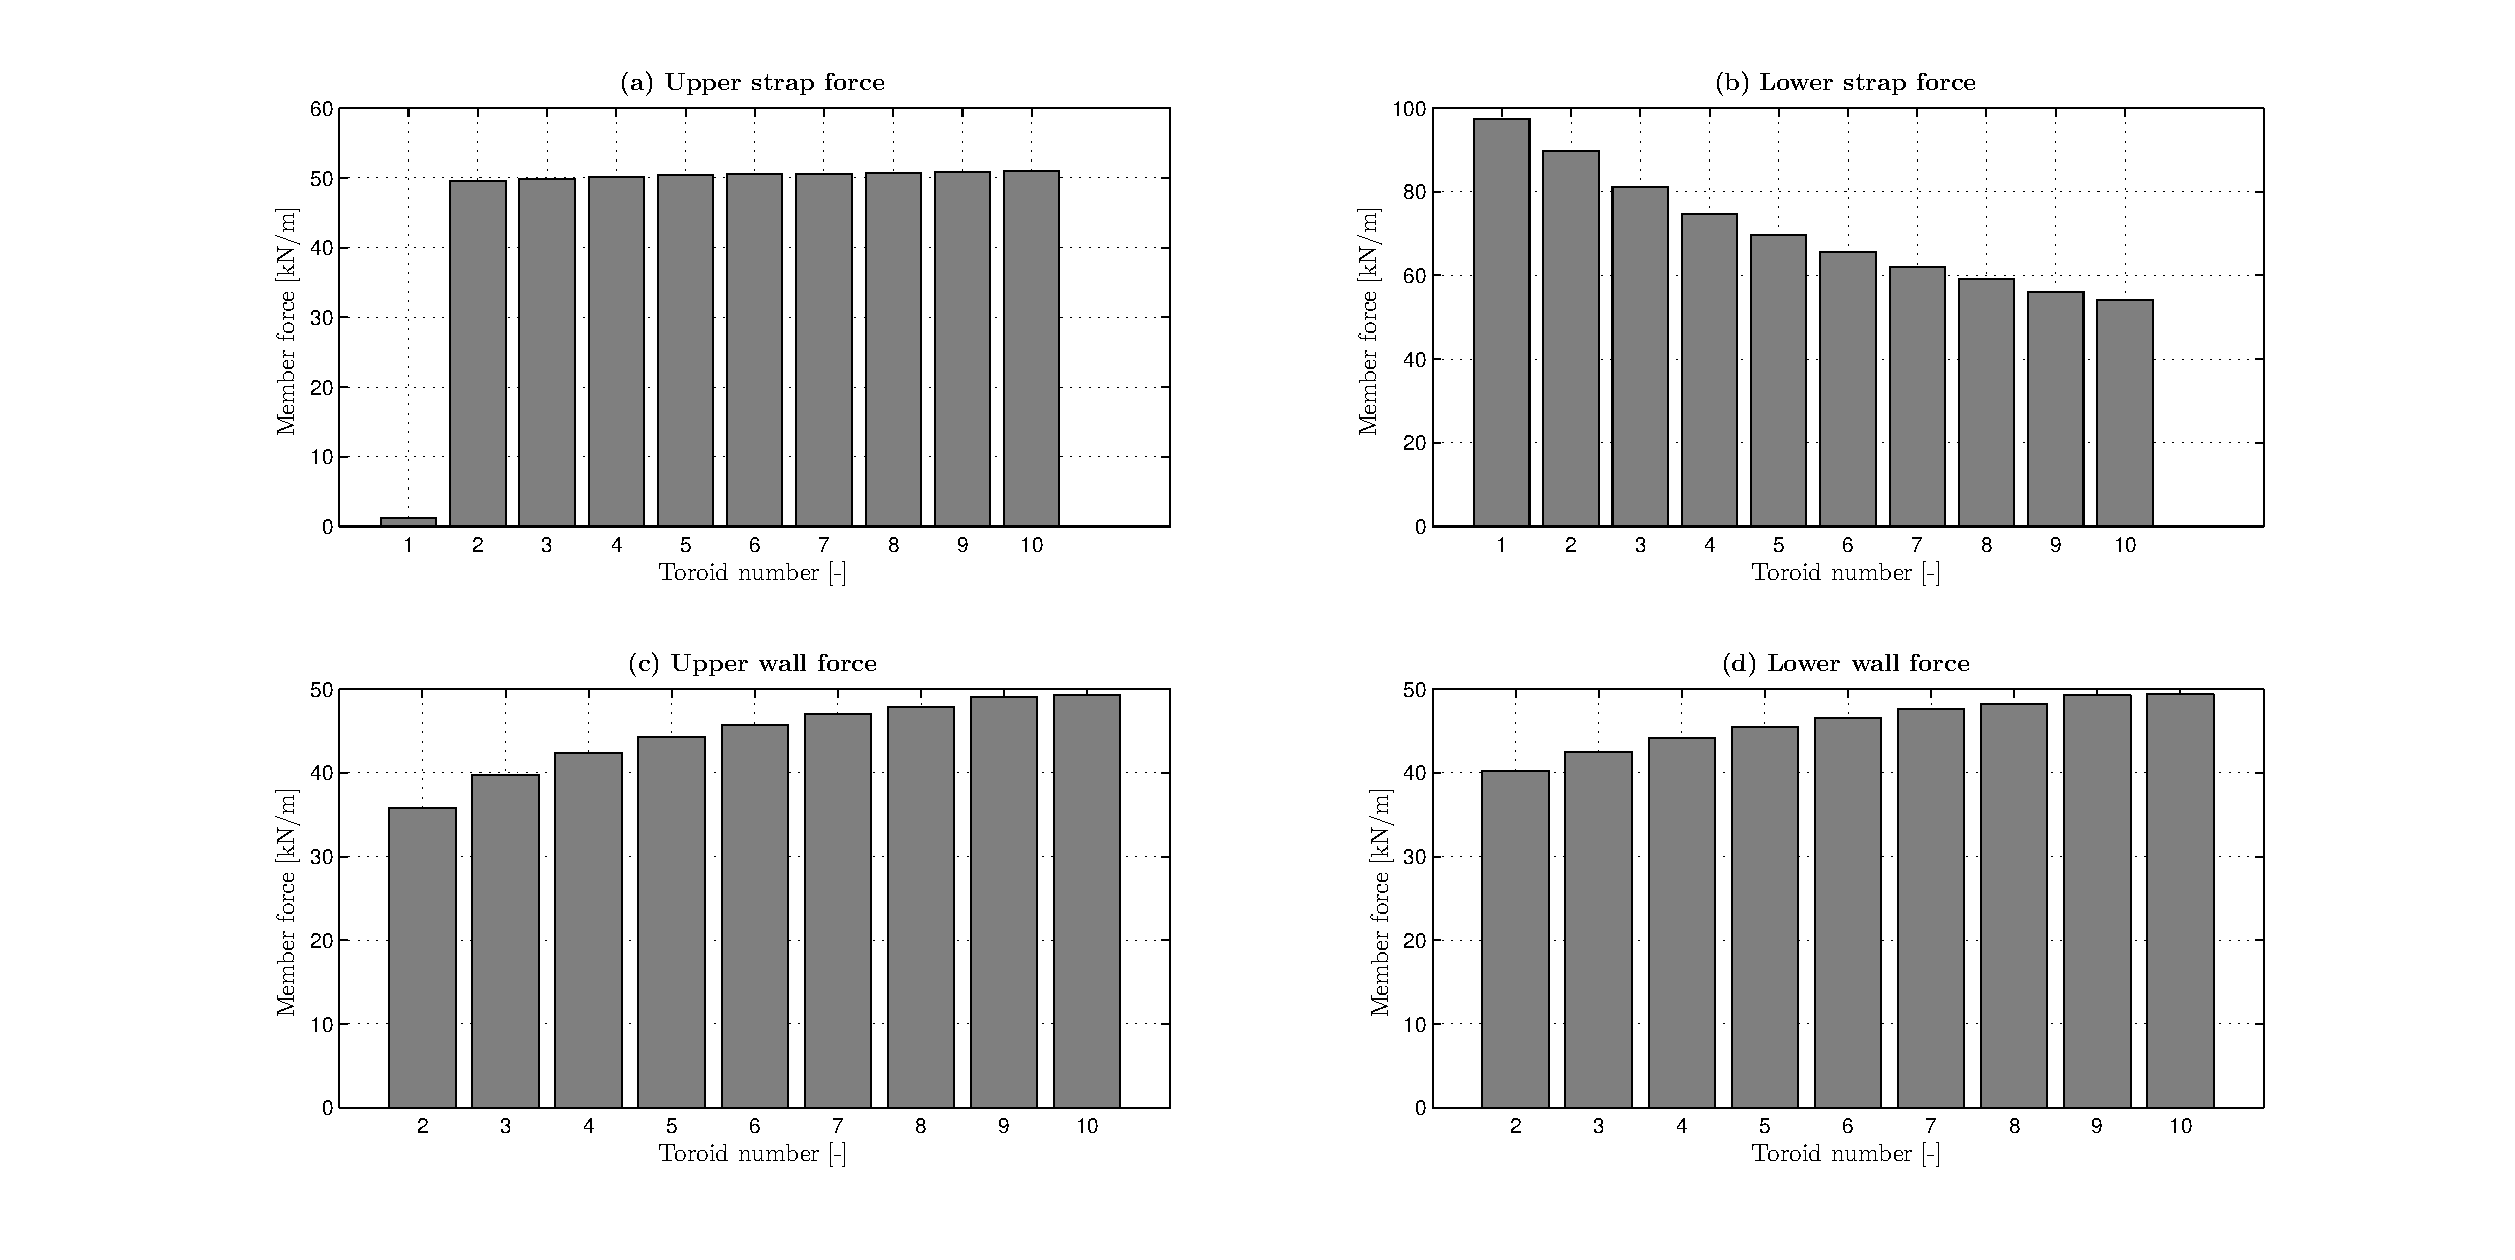
\includegraphics[width=1.2\textwidth]{./Figure/Structure/loads_long.eps}
		\caption{Cross-sectional running loads inflatable at maximum diameter}
		\label{fig:strucl}
\end{figure}
\begin{figure}[h!]
		\hspace{-16mm}
		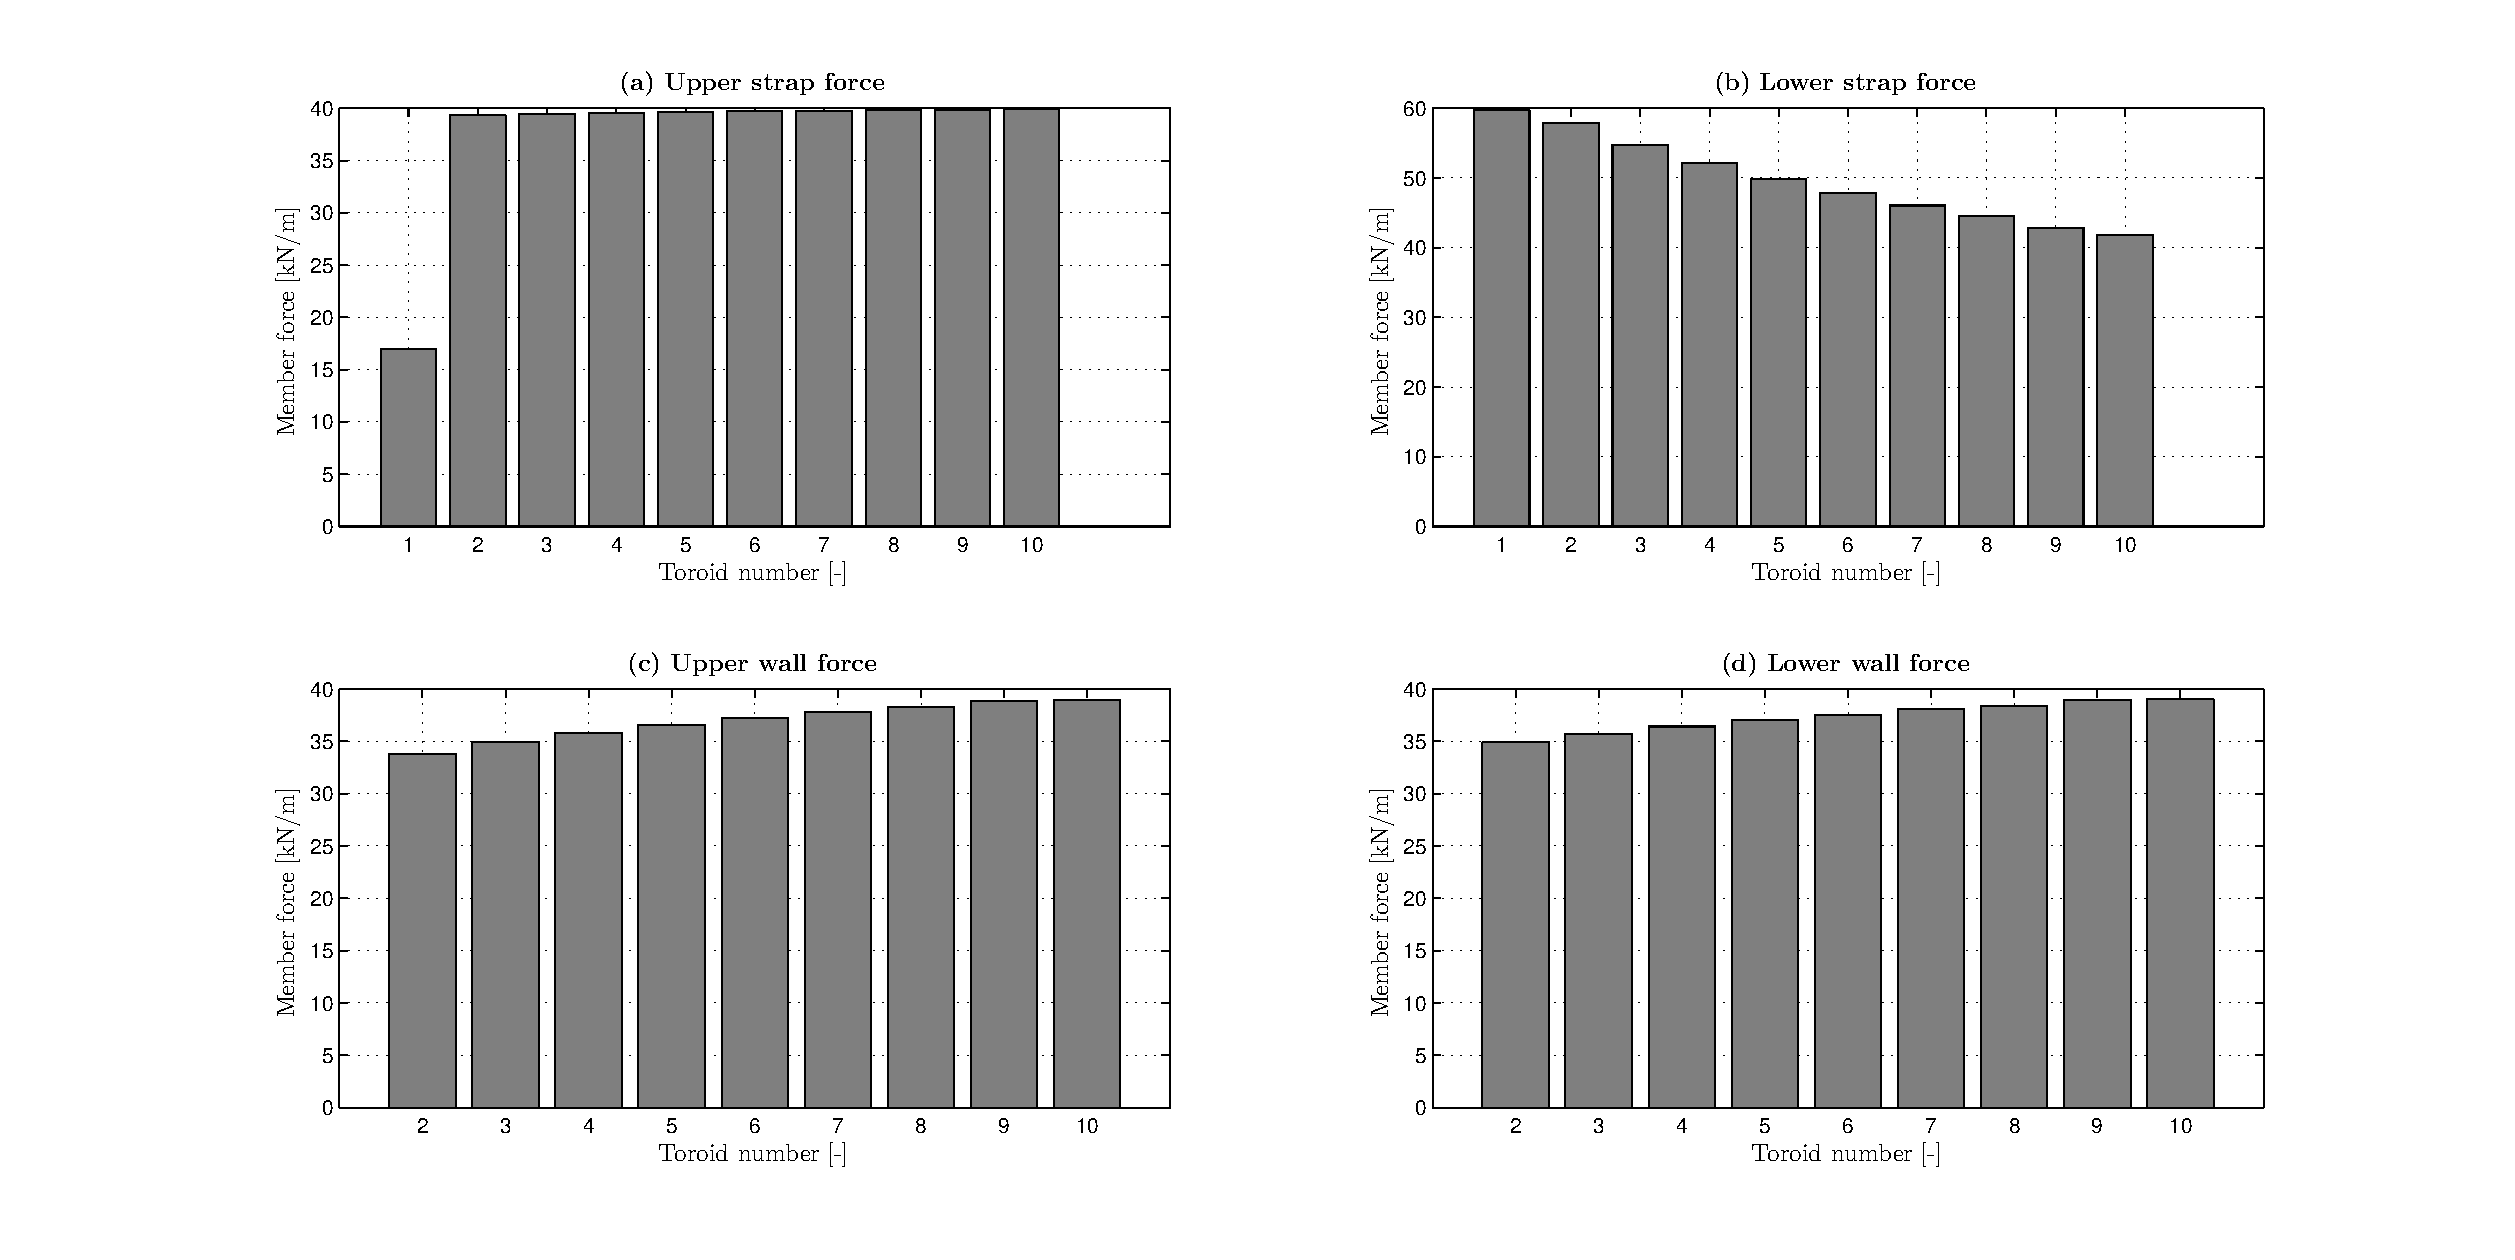
\includegraphics[width=1.2\textwidth]{./Figure/Structure/loads_short.eps}
		\caption{Cross-sectional running loads inflatable at minimum diameter}
		\label{fig:strucs}
\end{figure}

For an inflation pressure of 169 [$kPa$], required to bring all members into tension, structural loads are as obtained in Figures \ref{fig:strucl} and \ref{fig:strucs}. It can be observed that the maximum running load in the walls is 50 [$kN \cdot m^{-1}$]. Translating this to a stress by dividing through the 0.125 [$mm$] thickness yields a maximum stress of 400 [$MPa$], well below the tensile strength of 3 [$GPa$] for Kevlar 49. In the straps, the maximum running load is 100 [$kN \cdot m^{-1}$], translating to a 800 [$MPa$] stress. As such, the minimum gage thickness is well above the required thickness determined by preliminary load and stress analysis, taking into account a wide margin for material uncertainties, production deficiencies and unpredicted structural phenomena. The flexible material mass, given a uniform thickness of 0.125 [$mm$] for radial straps and toroid material, is 83 [$kg$].

Stitching of the fabrics making up the toroids is used for the joints of the inflatable, on one hand to join the toroids to each other and on the other hand to join the toroids to the radial straps. This is a method excellently suited, applied, tested and proven in the \gls{irve} missions \cite{Lindell2006,Hughes2011,Dillman2012}. Joints are thereby proven high-strength and suitable for space application and a stacked-toroid configuration.

For the load analysis, the ultimate load is calculated by multiplying with a \acrfull{fos} of 1.5. This \gls{fos} respects NASA standards for composite structures and accounts for uncertainties in the maximum external loading applied \cite{Technical2014}. 

To prevent Nitrogen gas from leaking, the structural Kevlar layers are coated with a gas barrier in the form of a 50 [$\mu m$] Upilex layer. This uniform thickness coating adds an estimated 25 [$kg$]. The thickness of this coating is feasible, in line with findings by Samareh and Miller \cite{Samareh2011,Miller2014} and available Upilex grades of 12.5, 25, 50, 75 and 125 [$\mu m$]\footnote{URL:\url{https://www.ube.com/content.php?pageid=81}. Accessed: 16-06-2015}$^{,}$\footnote{URL:\url{http://dasp.mem.odu.edu:8080/~deorbit_sp12/ref/UPILEXS\%20Data\%20sheet.pdf}. Accessed: 16-06-2015}.

%Typical driver for the use of fibres are the high mechanical properties, hence the application of Kevlar in the \gls{irve} missions \cite{Hughes2011}. Structural analyses proved the weight advantage of fibres over films in the case of \gls{irve}. In this case, however, density is leading and the mechanical properties of fibres are excessively high: their application would lead to an overdesign. This is reflected by Table \ref{tab:matfinal}. The flexible material mass achieved by Spectra 2000, expected to perform best of all fibres given its low density of 970 [$kg \cdot m^{-3}$], compared to Kevlar's 1440 [$kg \cdot m^{-3}$], is 20 [$kg$] lower than that achieved by Kevlar 49. 

%Films, however, provide a significant weight advantage. Upilex-25S and Kapton are films suitable for \gls{hiad} application \cite[p.59]{Balasooriyan2015b}. Upilex-25S is characterized by higher mechanical properties than Kapton, and due to the low minimum thickness for these films specific strength is the leading material property. The specific strength of Upilex-25S is nearly twice as high as that of Kapton \cite{Samareh2011} and this is reflected by its mass, nearly twice as low. The predominant advantage of using Upilex-25S over fibres is therefore directly reflected by the lower achievable structural mass, yielding a flexible material mass of 30 [$kg$].
%\begin{table}[h]
%\centering
%\caption{Comparison of flexible material mass for use of different materials}
%\label{tab:matfinal}
%\begin{tabular}{|l|l|l|l|l|}
%\hline
%{\bf Material}                        & Kevlar 49    & Spectra 2000 & Upilex-25S & Kapton \\ \hline
%{\bf Type}                            & Aramid fibre & Aramid fibre & Film       & Film   \\ \hline
%{\bf Flexible material mass {[}kg{]}} & 89             &  71          &  31          & 52        \\ \hline
%\end{tabular}
%\end{table}

%The weight advantage is predominantly effected by a lower minimum gage thickness for films. Minimum gage thickness for Upilex-25S is 25 [$\mu m$]\footnote{URL:\url{http://dasp.mem.odu.edu:8080/~deorbit_sp12/ref/UPILEXS\%20Data\%20sheet.pdf}. Accessed: 16-06-2015}.  The thickness required to withstand the loads is estimated at 0.025 [$mm$]



%As such, based on the discussion in Subsection \ref{subsec:strucsens} Spectra 2000 is expected to perform best given its low density of 970 [$kg \cdot m^{-3}$], compared to Kevlar's 1440 [$kg \cdot m^{-3}$]. This effects a 20 [$kg$] decrease in material mass by the use of Spectra 2000 as compared to the other materials in Figure \ref{fig:mat}, of comparable density with Kevlar 49. 

%Stitching of the fabrics making up the toroids is used for the joints of the inflatable, on one hand to join the toroids to each other and on the other hand to join the toroids to the radial straps. This is a method excellently suited, applied, tested and proven in the \gls{irve} missions \cite{Lindell2006,Hughes2011,Dillman2012}. Joints are thereby proven high-strength and suitable for space application and a stacked-toroid configuration.

%Structural integrity is provided by PBO Zylon AS, capable of retaining its strength at high temperature and able to withstand the required loads\footnote{URL:\url{http://www.toyobo-global.com/seihin/kc/pbo/zylon-p/bussei-p/technical.pdf}. Accessed: 15-06-2015}}. It has high specific properties, leading to a low structural mass, as follows from Figure \ref{fig:mat}. It performs only slightly worse than Spectra 2000 in the parametric mass model, but differences are slight (below 5 $\%$) and 
